\documentclass[final,t]{beamer} % beamer 3.10: do NOT use option hyperref={pdfpagelabels=false} !
%\documentclass[final,hyperref={pdfpagelabels=false}]{beamer} % beamer 3.07: get rid of beamer warnings
\usepackage[english]{babel}
\usepackage[utf8]{inputenc}
\usepackage{amsmath,amsthm, amssymb, latexsym}
%\usefonttheme[onlymath]{serif}

\useinnertheme[shadow]{rounded}
\usecolortheme{rose}
\usetheme{jdoc}
\setbeamertemplate{navigation symbols}{}

\boldmath
\usepackage[orientation=portrait,size=a1,scale=1.4]{beamerposter}                  % e.g. for DIN-A1 poster, with optional grid and debug output
%\usepackage[orientation=portrait,size=a0,scale=1.0,printer=rwth-glossy-uv.df]{beamerposter}   % e.g. for DIN-A0 poster with rwth-glossy-uv printer check
\usepackage{tikz}
\usetikzlibrary[decorations.pathmorphing]
\usepackage{ifthen}
\usepackage{tikz}
\usetikzlibrary{arrows,shapes}

\definecolor{lightgray}{rgb}{0.8,0.8,0.8}
\definecolor{lightgrey}{rgb}{0.8,0.8,0.8}

\tikzstyle{boxed ph}=[]
\tikzstyle{sort}=[fill=lightgray,rounded corners]
\tikzstyle{process}=[circle,draw,minimum size=15pt,fill=white,
font=\footnotesize,inner sep=1pt]
\tikzstyle{black process}=[process, fill=black,text=white, font=\bfseries]
\tikzstyle{gray process}=[process, draw=black, fill=lightgray]
\tikzstyle{current process}=[process, draw=black, fill=lightgray]
\tikzstyle{process box}=[white,draw=black,rounded corners]
\tikzstyle{tick label}=[font=\footnotesize]
\tikzstyle{tick}=[black,-]%,densely dotted]
\tikzstyle{hit}=[->,>=angle 45]
\tikzstyle{selfhit}=[min distance=30pt,curve to]
\tikzstyle{bounce}=[densely dotted,>=stealth',->]
\tikzstyle{hl}=[font=\bfseries,very thick]
\tikzstyle{hl2}=[hl]
\tikzstyle{nohl}=[font=\normalfont,thin]

\newcommand{\currentScope}{}
\newcommand{\currentSort}{}
\newcommand{\currentSortLabel}{}
\newcommand{\currentAlign}{}
\newcommand{\currentSize}{}

\newcounter{la}
\newcommand{\TSetSortLabel}[2]{
  \expandafter\repcommand\expandafter{\csname TUserSort@#1\endcsname}{#2}
}
\newcommand{\TSort}[4]{
  \renewcommand{\currentScope}{#1}
  \renewcommand{\currentSort}{#2}
  \renewcommand{\currentSize}{#3}
  \renewcommand{\currentAlign}{#4}
  \ifcsname TUserSort@\currentSort\endcsname
    \renewcommand{\currentSortLabel}{\csname TUserSort@\currentSort\endcsname}
  \else
    \renewcommand{\currentSortLabel}{\currentSort}
  \fi
  \begin{scope}[shift={\currentScope}]
  \ifthenelse{\equal{\currentAlign}{l}}{
    \filldraw[process box] (-0.5,-0.5) rectangle (0.5,\currentSize-0.5);
    \node[sort] at (-0.2,\currentSize-0.4) {\scriptsize\currentSortLabel};
   }{\ifthenelse{\equal{\currentAlign}{r}}{
     \filldraw[process box] (-0.5,-0.5) rectangle (0.5,\currentSize-0.5);
     \node[sort] at (0.2,\currentSize-0.4) {\scriptsize\currentSortLabel};
   }{
    \filldraw[process box] (-0.5,-0.5) rectangle (\scriptsize\currentSize-0.5,0.5);
    \ifthenelse{\equal{\currentAlign}{t}}{
      \node[sort,anchor=east] at (-0.3,0.2) {\scriptsize\currentSortLabel};
    }{
      \node[sort] at (-0.6,-0.2) {\scriptsize\currentSortLabel};
    }
   }}
  \setcounter{la}{\currentSize}
  \addtocounter{la}{-1}
  \foreach \i in {0,...,\value{la}} {
    \TProc{\i}
  }
  \end{scope}
}

\newcommand{\TTickProc}[2]{ % pos, label
  \ifthenelse{\equal{\currentAlign}{l}}{
    \draw[tick] (-0.6,#1) -- (-0.4,#1);
    \node[tick label, anchor=east] at (-0.55,#1) {#2};
   }{\ifthenelse{\equal{\currentAlign}{r}}{
    \draw[tick] (0.6,#1) -- (0.4,#1);
    \node[tick label, anchor=west] at (0.55,#1) {#2};
   }{
    \ifthenelse{\equal{\currentAlign}{t}}{
      \draw[tick] (#1,0.6) -- (#1,0.4);
      \node[tick label, anchor=south] at (#1,0.55) {#2};
    }{
      \draw[tick] (#1,-0.6) -- (#1,-0.4);
      \node[tick label, anchor=north] at (#1,-0.55) {#2};
    }
   }}
}
\newcommand{\TSetTick}[3]{
  \expandafter\repcommand\expandafter{\csname TUserTick@#1_#2\endcsname}{#3}
}

\newcommand{\myProc}[3]{
  \ifcsname TUserTick@\currentSort_#1\endcsname
    \TTickProc{#1}{\csname TUserTick@\currentSort_#1\endcsname}
  \else
    \TTickProc{#1}{#1}
  \fi
  \ifthenelse{\equal{\currentAlign}{l}\or\equal{\currentAlign}{r}}{
    \node[#2] (\currentSort_#1) at (0,#1) {#3};
  }{
    \node[#2] (\currentSort_#1) at (#1,0) {#3};
  }
}
\newcommand{\TSetProcStyle}[2]{
  \expandafter\repcommand\expandafter{\csname TUserProcStyle@#1\endcsname}{#2}
}
\newcommand{\TProc}[1]{
  \ifcsname TUserProcStyle@\currentSort_#1\endcsname
    \myProc{#1}{\csname TUserProcStyle@\currentSort_#1\endcsname}{}
  \else
    \myProc{#1}{process}{}
  \fi
}

\newcommand{\repcommand}[2]{
  \providecommand{#1}{#2}
  \renewcommand{#1}{#2}
}
\newcommand{\THit}[5]{
  \path[hit] (#1) edge[#2] (#3#4);
  \expandafter\repcommand\expandafter{\csname TBounce@#3@#5\endcsname}{#4}
}
\newcommand{\TBounce}[4]{
  (#1\csname TBounce@#1@#3\endcsname) edge[#2] (#3#4)
}

\newcommand{\TState}[1]{
  \foreach \proc in {#1} {
    \node[current process] (\proc) at (\proc.center) {};
  }
}




\spec{Informatique}
\labo{IRCCyN}
\equipe{MeForBio}

\title{Presentation of the Process Hitting framework and inference\\of Biological Regulatory Networks with Thomas parameters}
\author{Folschette Maxime}
\photo{Maxime.jpg}
\directeur{Olivier Roux}
\encadrant{Morgan Magnin}
\email{Maxime.Folschette@irccyn.ec-nantes.fr}

\newenvironment{myblock}[1]%
{\section{#1}\begin{block}{\thesection. #1}}%
{\end{block}}

\newlength{\columnheight}
\setlength{\columnheight}{150cm}



\usepackage{color}
\newcommand{\todo}[1]{\textbf{\textcolor{red}{[[#1]]}}}



\begin{document}
\begin{frame}{} 
\begin{columns}[T]
\begin{column}[b]{0.48\textwidth}
\parbox[t][\columnheight]{\textwidth}{% must be some better way to set the the height, width and textwidth simultaneously

% Colonne 1

\begin{myblock}{Introduction}
  \begin{itemize}
    \item Systems biology = studying and understanding of interactions inside biological systems
    \begin{itemize}
      \item cells, organisms…
      \item proteins/genes regulations
    \end{itemize}
    \item Biological systems are very complex
    \item They may over-approximate the desired behavior
  \end{itemize}
  \todo{image}
\end{myblock}

\begin{myblock}{Studying models}
  \begin{itemize}
    \item Models are often too large to be studied
    \item Usual model-checkers have to compute all states
  \end{itemize}
  %\todo{dessin model-checker}
  \begin{figure}
    \definecolor{darkred}{rgb}{0.5,0,0}
    \definecolor{darkgreen}{rgb}{0,0.5,0}
    \definecolor{darkblue}{rgb}{0,0,0.5}
    \tikzstyle{bigedge}=[->, shorten <=10pt, shorten >=10pt, line width=.2cm]
    \tikzstyle{warn}=[rounded corners, draw=darkred, line width=.07em, align=center, text=red]
  \begin{tikzpicture}[line width=.05em]
    \node[ellipse, draw=darkgreen, decoration={coil}, decorate, align=center] (system) {Biological\\system};
    \node[rounded corners, draw=darkblue, right of=system, node distance=10cm, below=0.5cm] (model) {Model};
    \node[rounded corners, draw=gray, below of=model, node distance=10cm] (properties) {Properties};
    
    \path[transparent, bend right] (model) edge node[right] (e) {} (properties);
    \node[left of=e, left=.5cm, warn] (out)
      {Computation time = $\infty$\\Memory size = $\infty$};
    \path[warn] (out) edge (e);
    \path[bigedge, bend left] (system) edge (model);
    \path[bigedge, bend right] (model) edge (properties);
  \end{tikzpicture}
  \end{figure}
\end{myblock}

\begin{myblock}{The Process Hitting framework}
  \begin{itemize}
    \item Recent framework well-adapted to large-scale models
    \item Atomistic representation of actions
    \item Very efficient reachability approximations (ms)
    \item Can handle models with hundreds of components
  \end{itemize}
  \todo{dessin PH + approx}
\end{myblock}

}
\end{column}
\begin{column}{0.48\textwidth}
\parbox[t][\columnheight]{\textwidth}{ % must be some better way to set the the height, width and textwidth simultaneously

% Colonne 2
\vspace*{.52cm}

\begin{myblock}{Translating PH models to Thomas modeling}
  \begin{itemize}
    \item More widespread representation of models after atomistic refining and study in PH
    \item PH = atomistic actions between processes
    \item Thomas = global actions between components
    \item Method: exhaustive search of interactions
  \end{itemize}
  \begin{centering}
  \begin{figure}
    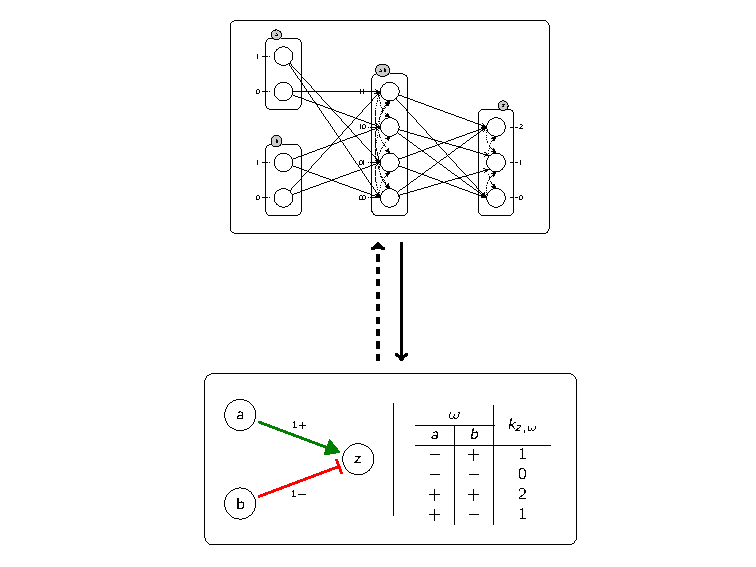
\includegraphics[scale=2.5,trim=2.5cm 0cm 2.1cm 0cm,clip=true]{ex-inf.pdf}
  \end{figure}
  \end{centering}
\end{myblock}

\begin{myblock}{Efficiently study Thomas models (?)}
  \todo{?}
\end{myblock}

\begin{myblock}{Conclusion}
  \begin{itemize}
    \item Formal translation PH $\rightarrow$ Thomas
    \item Implemented into the Pint library
    \item Efficient results on big models (20 \& 40 genes)
  \end{itemize}
  \todo{Table résultats}
\end{myblock}

}
\end{column}
\end{columns}

%\parbox[t][\columnheight]{\textwidth}{ % must be some better way to set the the height, width and textwidth simultaneously
\vspace*{-100cm}
xyzezfzefezfez xyzezfzefezfez xyzezfzefezfez xyzezfzefezfez 
%}

\end{frame}
\end{document}
